% ------------------------------------------------------------
\section{Calendar Week}
% ------------------------------------------------------------
% --------------------------------------------------- Slide --
\subsection{CW 30}
% ------------------------------------------------------------
\begin{frame}
  \frametitle{Review CW 30}
	\begin{itemize}
		\item Registration to Workshop "Literatursuche und -verwaltung fuer Doktoranden" at the MHH library. Presence planned at MHH in CW 38 (Friday, 25th September). - \textcolor{green}{Done}. Plan: 
		\begin{itemize}
			\item Participation in Workshop from 10h-12h.
			\item Work in the office in the afternoon.
			\item Eventually clarify any formalities.
		\end{itemize}			
		\item Inquiry regarding "Remote Access" -> Answer from IT: New ticket (855833) created, Citrix Server to be installed at MHH PC. Still no confirmed due date.  - \textcolor{yellow}{In Work} 
		\item Added possibility of multi-steps (for multiple loads and corresponding load cycles, still missing for multiple lengths) to created script. Objective: calculate and accumulate damage due to different loads in a single run of the script. First results obtained, see figure in next slide. - \textcolor{yellow}{In Work} 
	\end{itemize}
\end{frame}

\begin{frame}
  \frametitle{Review CW 30 - Model with Multi-Steps (compare with CW26)}
	\begin{figure}
		%\centering
		\subfigure{
		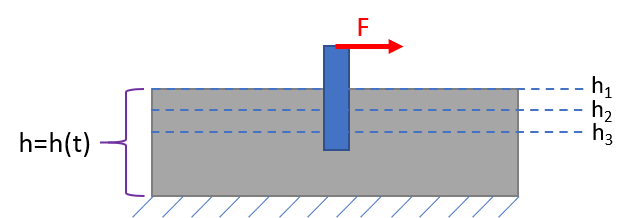
\includegraphics[width=0.45\textwidth]{pictures/CW26_1}
		}
		%\quad
		\subfigure{
		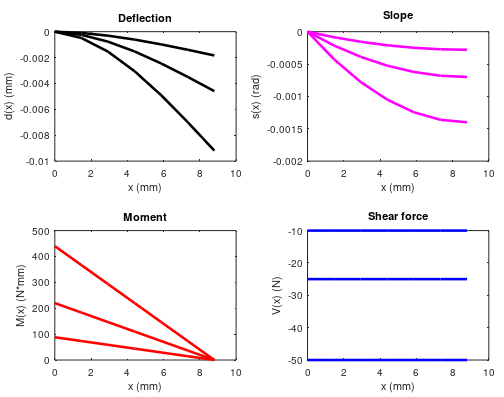
\includegraphics[width=0.45\textwidth]{pictures/CW30}
		}
	\end{figure}
\end{frame}

% ------------------------------------------------------------
% --------------------------------------------------- Slide --
\subsection{CW 31}
% ------------------------------------------------------------
% ------------------------------------------------------------
\begin{frame}
  \frametitle{Outlook CW 31}
	\begin{itemize}
		\item Continue work on adding possibility of multi-steps to created script. Add possibility of automatic variation of length (i.e., h = h(t)). Objective: calculate and accumulate damage due to different lengths in a single run of the script.
	\end{itemize}
\end{frame}
% --------------------------------------------------- Slide --

